\documentclass{beamer}

\usetheme{Madrid} % Singapore, Madrid, Ilmenau, CambridgeUS
\setbeamertemplate{navigation symbols}{}

% --- Colores personalizados ---
\definecolor{unahurverde}{HTML}{005C5C}
\definecolor{unahurgris}{HTML}{EAEAEA}
\setbeamercolor{structure}{fg=unahurverde}
\setbeamercolor{frametitle}{bg=unahurverde, fg=white}
\setbeamercolor{title}{fg=unahurverde}
\setbeamercolor{block title}{bg=unahurverde, fg=white}
\setbeamercolor{block body}{bg=unahurgris, fg=black}

% --- Logo en esquina superior derecha ---
\addtobeamertemplate{frametitle}{}{%
	\begin{textblock*}{3cm}(11.88cm,0.12cm)
		
\includegraphics[height=0.7cm]{logo_unahur.png}
	\end{textblock*}
}

\setbeamertemplate{caption}[numbered]


\usepackage[utf8]{inputenc}
\usepackage[spanish]{babel}
\usepackage{graphicx}
\usepackage{ragged2e}
\usepackage[table]{xcolor}
\usepackage{listings}
\usepackage{caption}
%\usepackage{enumitem}
\usepackage[absolute,overlay]{textpos} % Necesario para el logo

\usefonttheme[onlymath]{serif}

\definecolor{codegray}{rgb}{0.5,0.5,0.5}
\definecolor{backcolor}{rgb}{0.95,0.95,0.95}
\definecolor{verdecelda}{HTML}{B7CBA6}
\definecolor{rojocelda}{HTML}{FF9999}
\definecolor{lightgray}{gray}{0.6}

\definecolor{codebg}{rgb}{0.95,0.97,0.98}       % fondo celeste muy suave
\definecolor{codecomment}{rgb}{0.42,0.55,0.34}  % verde oliva suave y cursiva
\definecolor{codekeyword}{rgb}{0.0,0.45,0.73}    % azul turquesa
\definecolor{codestring}{rgb}{0.78,0.36,0.14}   % naranja marrón claro
\definecolor{codenumber}{rgb}{0.5,0.5,0.5}      % gris numeración
\definecolor{coderule}{rgb}{0.7,0.8,0.9}        % borde celeste suave

\lstdefinestyle{mystyle}{
	backgroundcolor=\color{codebg},
	commentstyle=\color{codecomment},
	keywordstyle=\color{codekeyword}\bfseries,
	stringstyle=\color{codestring},
	numberstyle=\tiny\color{codenumber},
	basicstyle=\ttfamily\footnotesize,
	breaklines=true,
	captionpos=b,
	keepspaces=true,
	numbersep=7pt,
	showspaces=false,
	showstringspaces=false,
	showtabs=false,
	tabsize=2,
	inputencoding=utf8,
	extendedchars=true,
	frame=single,
	rulecolor=\color{coderule},
	numbers=none,
	xleftmargin=10pt,
	literate={π}{{$\pi$}}1 {θ}{{$\theta$}}1 {μ}{{$\mu$}}1 {β}{{$\beta$}}1 {η}{{$\eta$}}1 {δ}{{$\delta$}}1 {Δ}{{$\Delta$}}1
	{á}{{\'a}}1 {é}{{\'e}}1 {í}{{\'i}}1 {ó}{{\'o}}1 {ú}{{\'u}}1
	{Á}{{\'A}}1 {É}{{\'E}}1 {Í}{{\'I}}1 {Ó}{{\'O}}1 {Ú}{{\'U}}1
	{ñ}{{\~n}}1 {Ñ}{{\~N}}1 {ζ}{{$\zeta$}}1
}

\lstset{style=mystyle}

\lstset{
	language=Python,
	emph={self, escalar_255, aplicar_umbralizacion, aplicar_magnitud_del_gradiente, aplicar_filtro, encontrar_cruces_por_cero, encontrar_cruces_por_cero_pendiente}, emphstyle=\color{purple}\bfseries,
	emph={[2]np.ndarray, np, sqrt, sum, ndarray, zeros_like, shape, zeros, copy, exp, newaxis},
	emphstyle={[2]\color{teal}\bfseries},
}

\title{Trabajo Práctico 3 Procesamiento de Imágenes y Visión por Computadora}
\author{Matías Cisnero}
\date{6 de Noviembre de 2025}

\begin{document}

% Portada
\begin{frame}
	\centering
	
\includegraphics[width=0.25\textwidth]{UNAHUR.png}
	\vfill
	{\huge \textbf{Trabajo Práctico 3}}\\[0.2cm]
	{\Large Procesamiento de Imágenes y Visión por Computadora}\\
	\vfill
	{\large Matías Cisnero}\\
	{\small 6 de Noviembre de 2025}
\end{frame}

\section{Ejercicio 1}

\begin{frame}
	\begin{center}
		\textcolor{unahurverde}{\textbf{Consigna 1:}}
	\end{center}
	\justifying
	Implementar el detector de bordes de Canny. Aplicarlo a una imagen y a su versión contaminada con distintos tipo de ruido.
\end{frame}

\begin{frame}[fragile]{Estrategia}
	\justifying
	\begin{block}{Detecto de Canny}
		\begin{enumerate}
			\item Aplicar un filtro Gaussiano.
			\item Aplicar el método de Sobel para calcular aproximadamente el gradiente y con esto la Magnitud de Borde.
			\item Calcular el ángulo del gradiente.
			\item Discretizar los ángulos en 4 valores (0º, 45º, 90º, 135º).
			\item Realizar la supresión de no máximos.
			\item Aplicar umbralización con histéresis.
		\end{enumerate}
	\end{block}
	
	\vfill
	\footnotesize \textcolor{lightgray}{(*) Obviaremos el paso 1 y 2 porque ya lo hemos realizado anteriormente.}
\end{frame}

\begin{frame}[fragile]{Resultados}
	\justifying
	Al aplicar el \textcolor{unahurverde}{\textbf{Detector de Canny}} ($t_1 = 50, t_2 = 150$) sobre la imagen de la Figura~\ref{fig:ej1}, se obtuvo las imagen de borde visible en la Figura~\ref{fig:ej1a}.
	\vspace{0.3cm}
	
	\centering
	\begin{minipage}{0.4\linewidth}
		\centering
		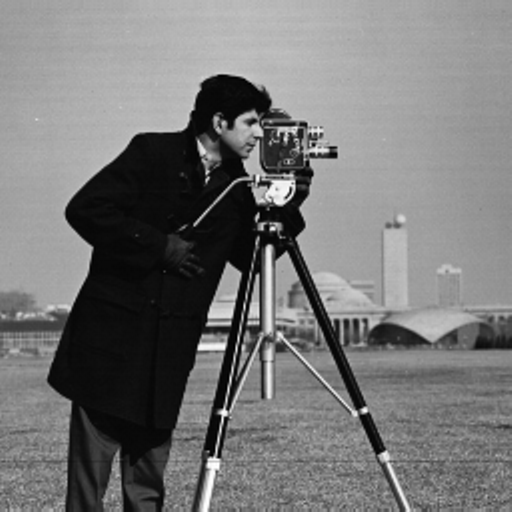
\includegraphics[width=\linewidth]{cameraman}
		\captionof{figure}{Original}
		\label{fig:ej1}
	\end{minipage}\hfill
	\begin{minipage}{0.4\linewidth}
		\centering
		
\includegraphics[width=\linewidth]{ej1a}
		\captionof{figure}{Imagen de borde}
		\label{fig:ej1a}
	\end{minipage}\hfill
	
	\vfill
	\footnotesize \textcolor{lightgray}{(*) Comentario.}
\end{frame}

\begin{frame}[fragile]{Resultados con ruido}
	\justifying
	Sobre la misma imagen original se aplicó el \textbf{Detector de Canny} a imágenes afectadas por distintos tipos de ruido:
	
	{\footnotesize
		\begin{itemize}
			\item Figuras~\ref{fig:canny_gauss} y~\ref{fig:canny_gauss_result}: ruido \textbf{Gaussiano} ($\sigma =$ 20, $\% =$ 40) con $t_1 = 50, t_2 = 150$.
			\item Figuras~\ref{fig:canny_syp} y~\ref{fig:canny_syp_result}: ruido \textbf{Sal y Pimienta} ($p =$ 10) con $t_1 = 40, t_2 = 220$.
		\end{itemize}
	}
	
	\vspace{0.3cm}
	
	\centering
	\begin{minipage}{0.24\linewidth}
		\centering
		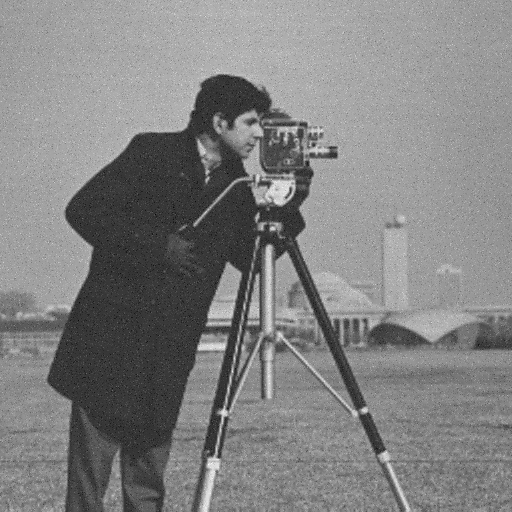
\includegraphics[width=\linewidth]{cameraman_gauss}
		\captionof{figure}{Ruido Gaussiano}
		\label{fig:canny_gauss}
	\end{minipage}\hfill
	\begin{minipage}{0.24\linewidth}
		\centering
		
\includegraphics[width=\linewidth]{ej1b}
		\captionof{figure}{Canny (Gauss)}
		\label{fig:canny_gauss_result}
	\end{minipage}\hfill
	\begin{minipage}{0.24\linewidth}
		\centering
		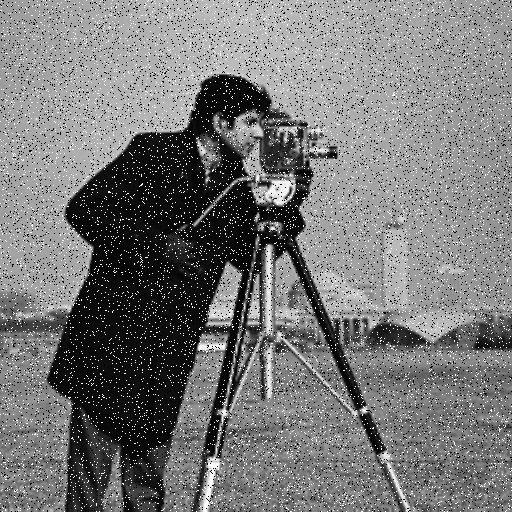
\includegraphics[width=\linewidth]{cameraman_syp}
		\captionof{figure}{Ruido SyP}
		\label{fig:canny_syp}
	\end{minipage}\hfill
	\begin{minipage}{0.24\linewidth}
		\centering
		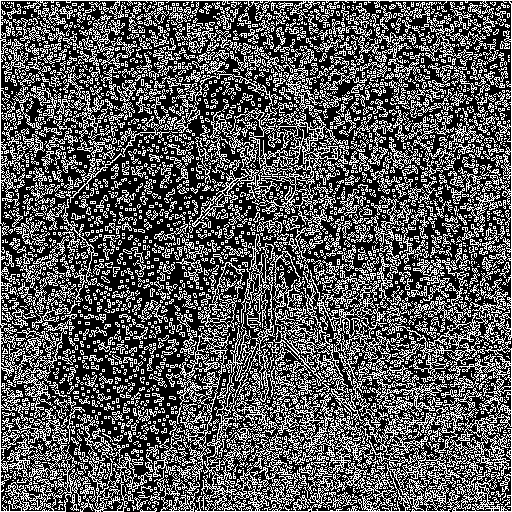
\includegraphics[width=\linewidth]{ej1c}
		\captionof{figure}{Canny (SyP)}
		\label{fig:canny_syp_result}
	\end{minipage}
\end{frame}


\section{Ejercicio 2}

\begin{frame}
	\begin{center}
		\textcolor{unahurverde}{\textbf{Consigna 2:}}
	\end{center}
	\justifying
	Implementar el Método de Smallest Univaluate Assimilating Nucleus (SUSAN) para:
	\begin{enumerate}
		\item Detección de bordes.
		\item Detección de esquinas.
	\end{enumerate}
	Aplicarlos a la imagen Test y a su versión contaminada.
\end{frame}

\begin{frame}[fragile]{Resultados}
	\justifying
	Al aplicar el \textcolor{unahurverde}{\textbf{Método de SUSAN}} sobre la imagen Test de la Figura~\ref{fig:ej2}, se obtuvieron las imágenes con bordes y esquinas resaltados visibles en la Figura~\ref{fig:ej2a} y Figura~\ref{fig:ej2b}.
	\vspace{0.3cm}
	
	\centering
	\begin{minipage}{0.3\linewidth}
		\centering
		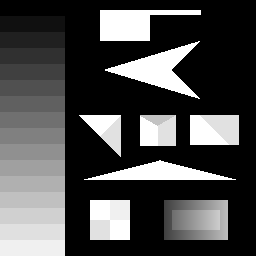
\includegraphics[width=\linewidth]{test}
		\captionof{figure}{Original}
		\label{fig:ej2}
	\end{minipage}\hfill
	\begin{minipage}{0.3\linewidth}
		\centering
		
\includegraphics[width=\linewidth]{ej2a}
		\captionof{figure}{Bordes}
		\label{fig:ej2a}
	\end{minipage}\hfill
	\begin{minipage}{0.3\linewidth}
		\centering
		
\includegraphics[width=\linewidth]{ej2b}
		\captionof{figure}{Esquinas}
		\label{fig:ej2b}
	\end{minipage}
	
	\vfill
	\footnotesize \textcolor{lightgray}{(*) c.}
\end{frame}

\begin{frame}[fragile]{Resultados con ruido}
	\justifying
	Al aplicar el \textcolor{unahurverde}{\textbf{Método de SUSAN}} sobre la imagen Test de la Figura~\ref{fig:ej2_gauss} con ruido Gaussiano ($\%=40, \sigma=20$), se obtuvieron las imágenes con bordes y esquinas resaltados visibles en la Figura~\ref{fig:ej2a_gauss} y Figura~\ref{fig:ej2b_gauss}.
	\vspace{0.3cm}
	
	\centering
	\begin{minipage}{0.3\linewidth}
		\centering
		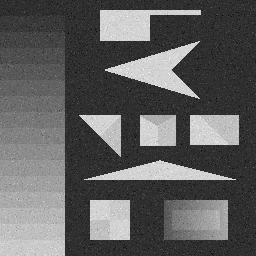
\includegraphics[width=\linewidth]{test_gauss}
		\captionof{figure}{Ruido Gauss}
		\label{fig:ej2_gauss}
	\end{minipage}\hfill
	\begin{minipage}{0.3\linewidth}
		\centering
		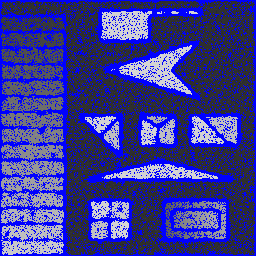
\includegraphics[width=\linewidth]{ej2a_gauss}
		\captionof{figure}{Bordes}
		\label{fig:ej2a_gauss}
	\end{minipage}\hfill
	\begin{minipage}{0.3\linewidth}
		\centering
		
\includegraphics[width=\linewidth]{ej2b_gauss}
		\captionof{figure}{Esquinas}
		\label{fig:ej2b_gauss}
	\end{minipage}
	
	\vfill
	\footnotesize \textcolor{lightgray}{(*) c.}
\end{frame}

\section{Ejercicio 3}

\begin{frame}
	\begin{center}
		\textcolor{unahurverde}{\textbf{Consigna 3:}}
	\end{center}
	\justifying
	 Implementar la transformada de Hough para detectar rectas y aplicarla a la imagen Test y a su versión contaminada.
\end{frame}

\section{Ejercicio 4}

\begin{frame}
	\begin{center}
		\textcolor{unahurverde}{\textbf{Consigna 4:}}
	\end{center}
	\justifying
	 Implementar el método de segmentación basado en conjuntos de nivel e intercambio de pixels y aplicarlo a imágenes estáticas. Aplicarlo también a imágenes contaminadas con ruido. Analizar para que tipo de imágenes es conveniente utilizar el método.
\end{frame}

\begin{frame}[fragile]{Operadores de gradiente}
	\justifying
	
	Los operadores de gradiente se basan en calcular estimaciones del \textbf{gradiente}.
	\begin{block}{En imágenes se calcula como:}
		$I : \Re^2 \rightarrow [0,...,255]$
		\[
		\nabla I = (I_x, I_y)
		\]
		El vector $\nabla I$ representa el gradiente de la imagen, y para cada píxel apunta en la dirección de mayor cambio de intensidad.
	\end{block}
	
	$I_x$ y $I_y$ se pueden aproximar con los operadores de \textbf{Prewitt} y de \textbf{Sobel}.
	
	\begin{block}{Magnitud del gradiente}
		Para cada píxel se calcula:
		\[
		|\nabla I|= \sqrt{I^2_x + I^2_y}
		\]
		Este valor indica la magnitud del cambio en la intensidad.
	\end{block}
	
\end{frame}

\begin{frame}[fragile]{Código: Magnitud del gradiente}
	\justifying
	El código detectar los bordes de una imagen mediante los operadores de gradiente es:
	\begin{lstlisting}[language=Python]
		def aplicar_magnitud_del_gradiente(imagen_np: np.ndarray, func_filtro1, func_filtro2) -> np.ndarray:
		
		ix = aplicar_filtro(imagen_np, func_filtro=func_filtro1, modo=2)
		iy= aplicar_filtro(imagen_np, func_filtro=func_filtro2, modo=2)
		
		magnitud = np.sqrt((ix**2)+(iy**2))
		
		resultado_np = escalar_255(magnitud)
		
		return resultado_np
	\end{lstlisting}
\end{frame}

\section{Repositorio}

\begin{frame}{Repositorio de GitHub}
	\justifying
	Todo el código y los resultados de este trabajo están disponibles en mi repositorio de GitHub: 
	
	\vspace{0.5cm}
	\centering
	\href{https://github.com/matias-cisnero/procesamiento_imagenes}{\textcolor{unahurverde}{\textbf{https://github.com/matias-cisnero/procesamiento\_imagenes}}}
\end{frame}

\section{Bibliografía}

\begin{frame}{Referencias}
	\tiny
	\begin{thebibliography}{10}
		\beamertemplateonlinebibitems
		\bibitem{numpy-broadcasting}
		NumPy Documentation: Broadcasting. 
		\newblock \url{https://numpy.org/doc/stable/user/basics.broadcasting.html}
		
		\bibitem{wikimedia-leucanthemum}
		Imagen \textit{“Leucanthemum vulgare Blüte”} por Mariofan13. 
		\newblock Wikimedia Commons. Licencia \textit{CC BY-SA 3.0 Unported}. 
		\newblock \href{https://commons.wikimedia.org/wiki/File:Leucanthemum_vulgare_Bl\%C3\%BCte.JPG}{Ver imagen en Wikimedia Commons}
		
		\beamertemplatebookbibitems
		\bibitem{digital-image-processing}
		Gonzalez, R. and Woods, R. (2018). Digital Image Processing. Pearson Education 4th Edition, New York.
	\end{thebibliography}
\end{frame}

\begin{frame}{}
	\centering
	{\huge ¡Gracias!}\\
	\vspace{1cm}
	
\includegraphics[width=0.2\textwidth]{UNAHUR.png}
\end{frame}
	
\end{document}
